\documentclass[10pt]{article}
\usepackage[utf8]{inputenc}
\usepackage[T1]{fontenc}
\usepackage{amsmath}
\usepackage{amsfonts}
\usepackage{amssymb}
\usepackage[version=4]{mhchem}
\usepackage{stmaryrd}
\usepackage{graphicx}
\usepackage[export]{adjustbox}
\graphicspath{ {./images/} }

\title{Università degli studi di Catania 
 Corso di Laurea in Fisica - Primo livello - A.A. 2021-2022 
 Esame di informatica - 7 gennaio 2022 
 Prof. Marco Russo }

\author{}
\date{}


\begin{document}
\maketitle
Occorre scrivere un programma in \(\mathrm{C}\) che esegue un filtraggio di una serie numerica \(d\). Questo filtraggio deve essere calcolato tramite una finestra mobile caratterizzata da \(n_{w}\) valori. La serie numerica \(d\) si trova nel file dati.txt. Tale file contiene il numero di campioni seguito dai campioni stessi. Nel file tutti i valori (compreso il loro numero) sono rappresentati in notazione scientifica e si trovano uno per ciascuna riga. I valori della finestra mobile sono ubicati nel file f.txt la cui conformazione è la medesima del precedente.

All'acquisizione su array quasi-statico sia dei campioni che dei valori del filtro occorre calcolare e stampare su video (in entrambi i casi) il loro valore minimo e quello massimo.

Successivamente, occorre generare un nuovo array quasi-statico in cui vengono immessi i valori filtrati \(d f_{i}\). Considerato che la dimensione \(n_{w}\) della finestra è sempre dispari e fissato \(n_{2}\) il risultato della divisione intera di \(n_{w}\) per 2 , avremo che i primi e gli ultimi \(n_{2}\) valori dell'array filtrato devono essere posti a 0 . Per gli altri valori avremo che il valore \(d f_{i}\) sarà determinato dal prodotto scalare tra il vettore degli \(n_{w}\) valori del filtro e il vettore di medesima ampiezza di valori consecutivi di \(d\) con valore centrale pari proprio a \(d_{i}\), cioè:

\[
d f_{i}=\sum_{j=-n_{2}}^{n_{2}} w_{j+n_{2}} d_{i+j} .
\]

In ultimo, il programma deve chiedere da tastiera una soglia. A fronte di questa soglia, si devono individuare gli intervalli laddove i dati filtrati \(d f_{i}\) sono maggiori della soglia. Tra tutti questi intervalli occorre fornire in output quello più ampio ed i numeri dei campioni di inizio e fine di quest'intervallo. I campioni si intendono numerati a partire dal valore uno. Come di consueto è vietato l'uso di array statici.

La figura mostra i dati forniti dal docente come esempio.

Quindi se il file f.txt contiene:

\(5.00000000+00\)

\(1.00000000 e-01\)

\(1.00000000 e-01\)

\(1.00000000 \mathrm{e}-0\)

\(2.00000000 e-01\)

\(5.00000000 \mathrm{e}-01\)

Se diamo come soglia 0.5 avremo come output:

D\_min \(=0.00 \quad D \_\max =2.00\)

W\_min \(=0.10\) W\_max \(=0.50\)

Soglia: 0.5

L\_max \(=35\) Start \(=32 \quad\) End \(=66\)

Se invece diamo come soglia 0.2 avremo come output:

D\_min \(=0.00 \quad D \_\max =2.00\)

W\_min \(=0.10\) W\_max \(=0.50\)

Soglia: 0.2

\(L_{-} \max =70\) Start=3 End=72

Laddove i valori del filtro sono:

\begin{center}
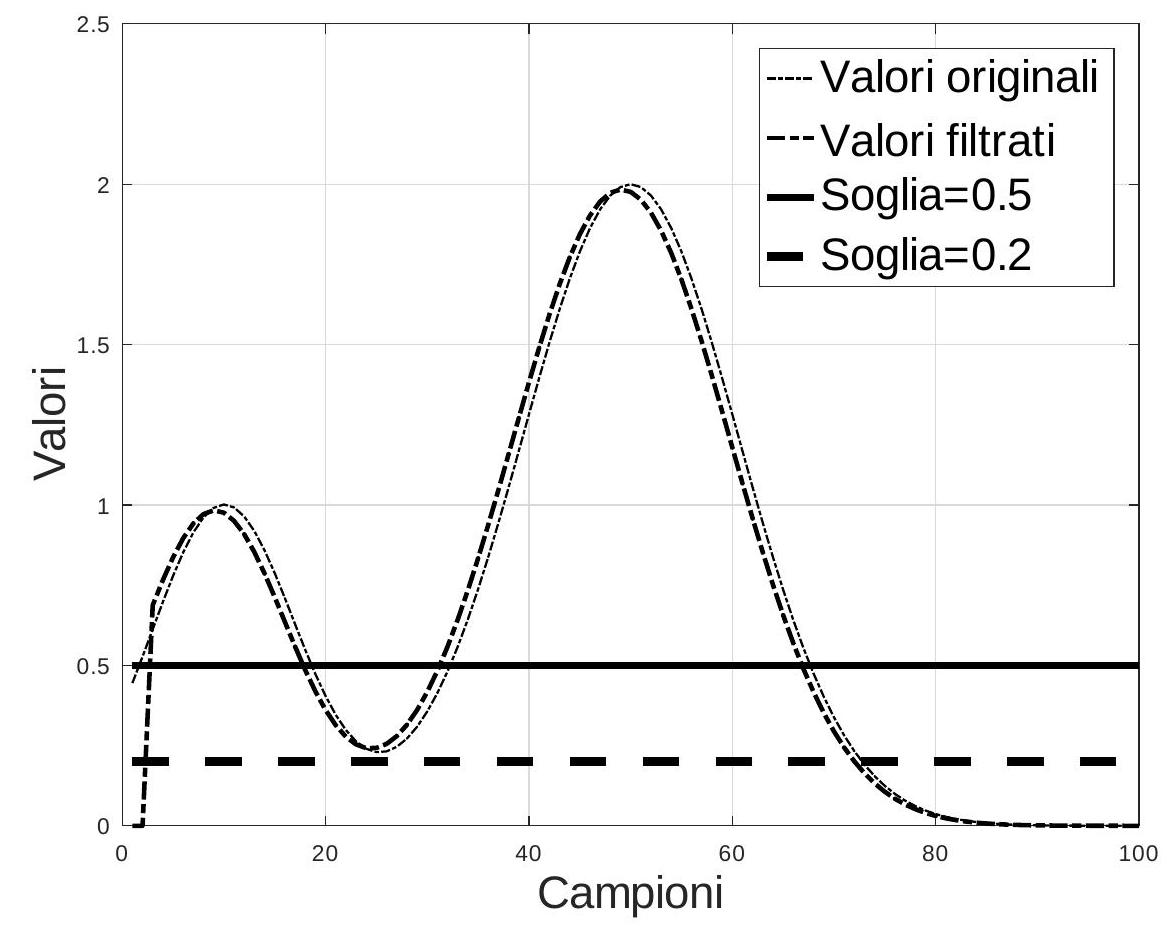
\includegraphics[max width=\textwidth]{2023_04_11_b7f0f4d0278d50ebd28ag-1}
\end{center}

Valutazione del compito.

\begin{center}
\begin{tabular}{|l|l|}
\hline
4 punti & Per l'acquisizione dei valori \(d_{i}\) \\
\hline
4 punti & Per l'acquisizione dei valori del filtro \(w_{i}\) \\
\hline
5 punti & Per il calcolo del minimo e del massimo \(d_{i}\) \\
\hline
5 punti & Per il calcolo del minimo e del massimo \(w_{i}\) \\
\hline
2 punti & Per l'acquisizione da tastiera della soglia \\
\hline
7 punti & Per la creazione ed il calcolo di \(d f\) \\
\hline
8 punti & Per la ricerca e stampa su video dei dati interenti l'intervallo cercato \\
\hline
\end{tabular}
\end{center}


\end{document}